\clearpage
\chapter{RESULTS AND DISCUSSIONS}

The integration of Moodle with the Namaste BHU application represents a significant milestone in enhancing the academic experience and administrative efficiency at Banaras Hindu University. Through meticulous deployment, configuration, and integration efforts, the project has successfully established a seamless connection between the two platforms, enabling students, faculty, and staff to access course materials, communicate, and collaborate more effectively.

\textbf{Moodle}\\
The deployment of Moodle on the Azure cloud infrastructure, along with the installation of essential plugins and extensions, has provided a robust and scalable learning management system for managing courses, resources, and activities. Moodle incorporates key features and functionalities, such as RESTful Protocol, Auth Userkey, and AirNotifier, to enhance accessibility, security, and communication within the platform.

The moodle is hosted at \href{http://20.174.1.153/moodle}{\texttt{http://20.174.1.153/moodle}} on an Azure Instance.

\begin{figure}[h]
    \centering
    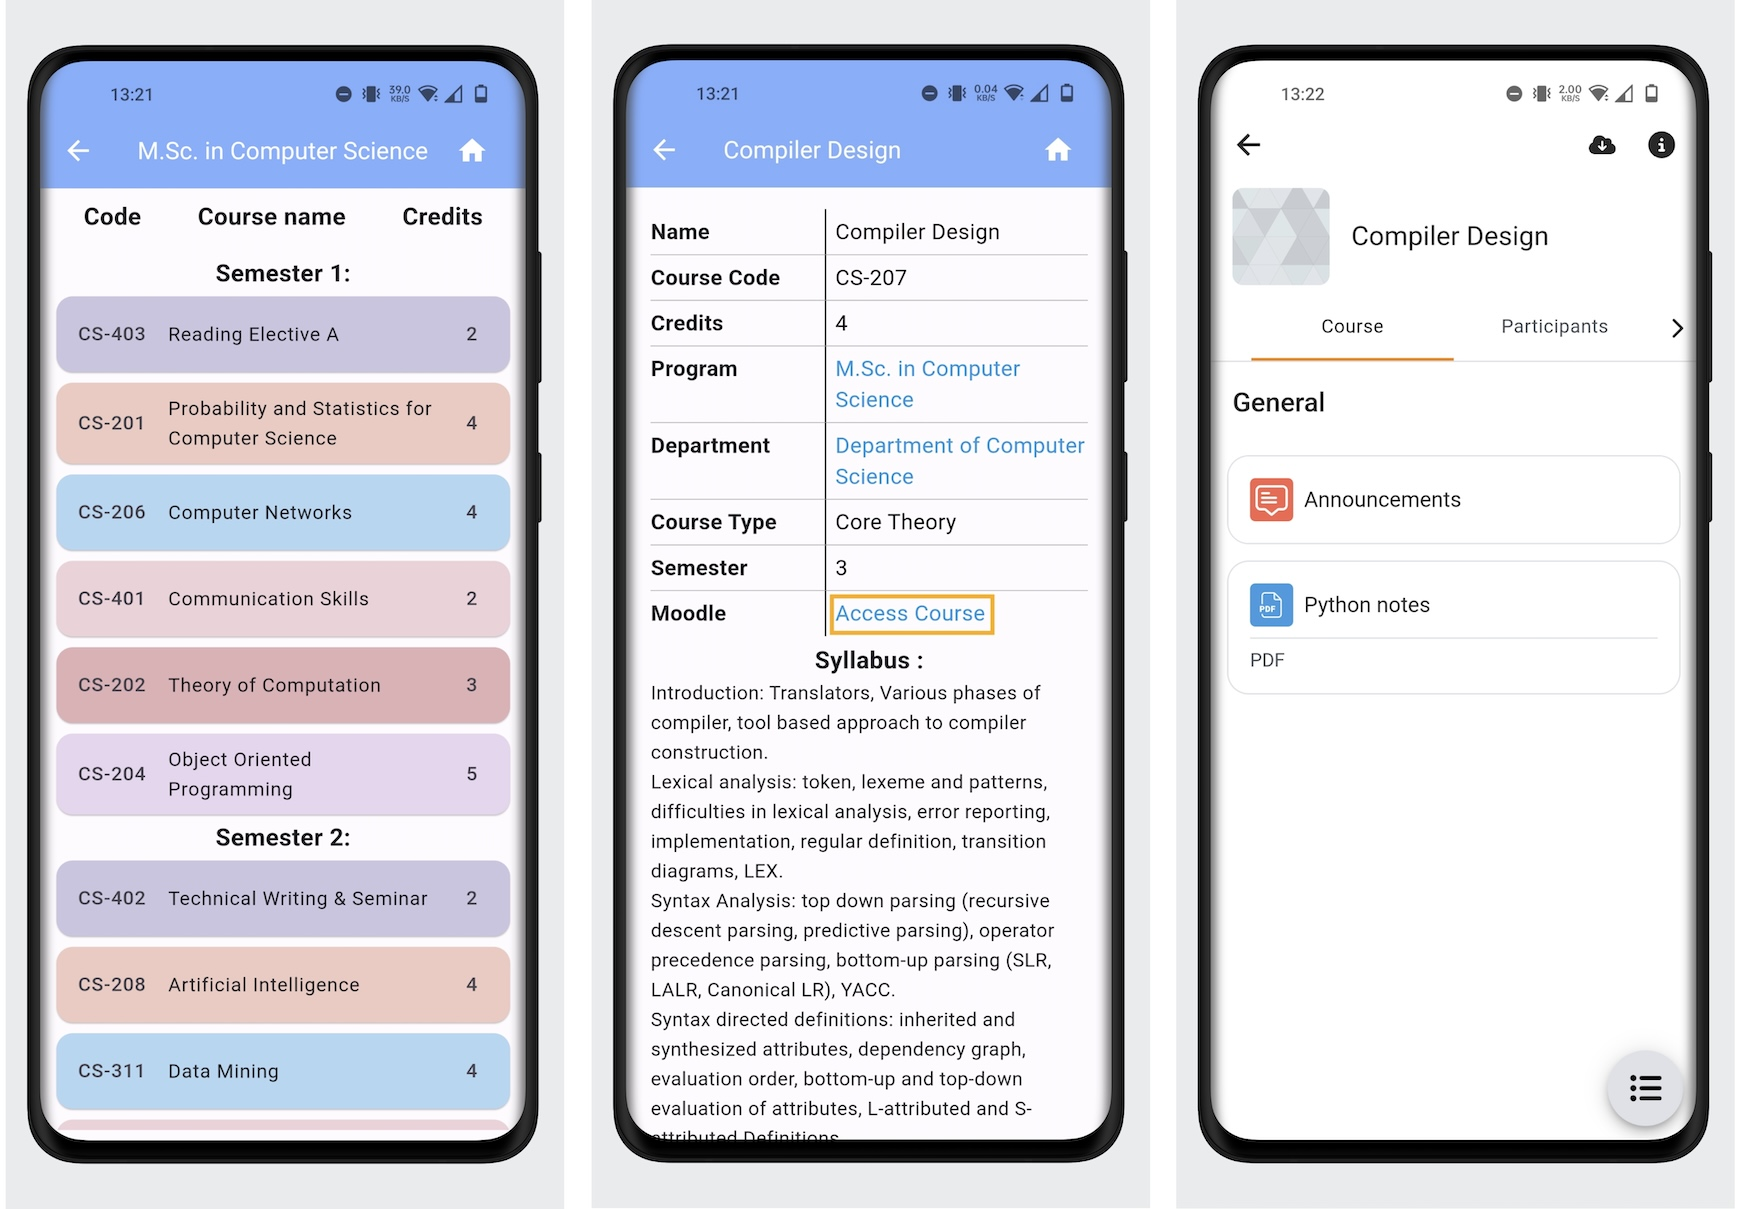
\includegraphics[width=\linewidth]{assets/img/result-opt.jpg}
    \caption{Final Application}
    \label{fig:result}
\end{figure}

\textbf{Namaste BHU}\\
The Namaste BHU Architecture underwent updates and enhancements to facilitate seamless integration with Moodle. New features and functionalities were introduced in Namaste BHU to support single sign-on (SSO) through deep linking of the Moodle Mobile App. The updated Namaste BHU application serves as a central hub for accessing Moodle content, enabling users to seamlessly navigate between the two platforms and engage with course materials, announcements, and discussions. In future it will also deliver notification from Moodle through Airnoitifier.
